\documentclass{article}

\usepackage[utf8]{inputenc}
\usepackage[T1]{fontenc}
\usepackage[a4paper, left=0cm, right=0cm, top=1cm, bottom=0cm]{geometry}
\usepackage{tikz}

\usetikzlibrary{calendar}

\begin{document}
\newcommand{\deadline}[2]{\draw (cal-#1) node[align=center]{#2};}

\newcommand{\daycode}{
  \node[shape=rectangle,
        draw=gray,
        minimum height=2cm,
        minimum width=2cm,
        anchor=center]{}
    ++(0, -0.1cm) node[anchor=center,name=\pgfcalendarsuggestedname]{}
    ++(-1cm, 0.8cm) node[anchor=west]{\tikzdaytext};
}

\begin{center}
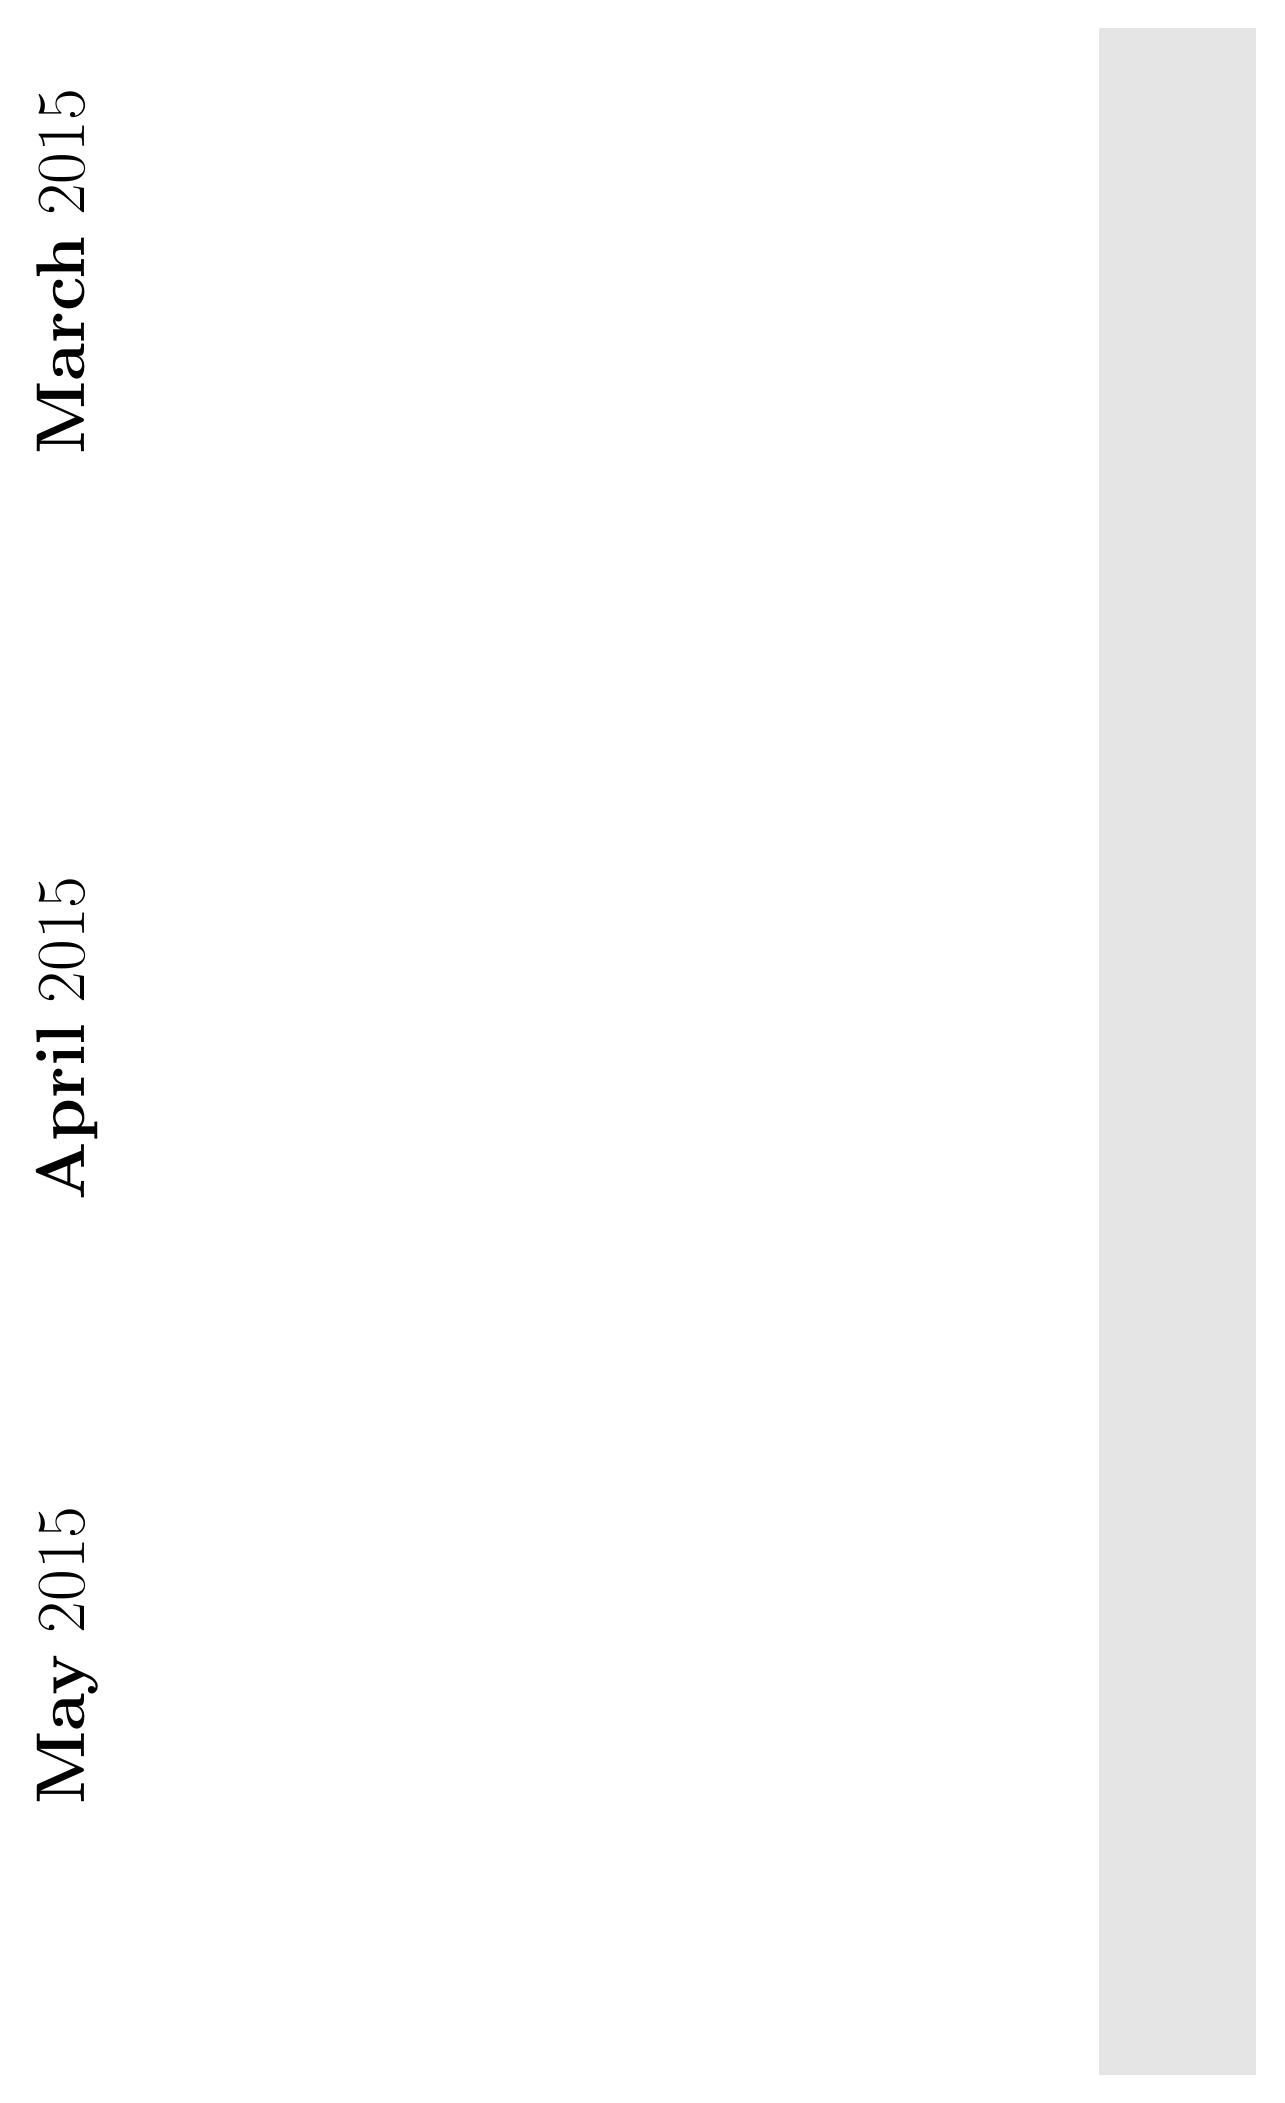
\begin{tikzpicture}
  \calendar (cal) [dates=2015-03-01 to 2015-05-30,
                   week list,
                   day yshift=2cm, day xshift=2cm,
                   day code=\daycode,
                   month label left vertical,
                   month code={\path ++(-1.2cm, 0) node[every month]{\Huge \tikzmonthtext};},
                   month yshift=0pt,
                   month text=\textbf{\%mt} \%y-]
    if (Sunday) {\fill[black!10] (-1cm,-1cm) rectangle (1cm,1cm);};

  \deadline{2015-03-09}{Stroemi}
  \deadline{2015-03-24}{Thermo2}
\end{tikzpicture}
\end{center}
\end{document}
